\label{delta_dist_donnees}

\subsubsection{Représentations géométriques}
\par Les modèles que l'on entraîne devant prédire la géométrie des molécules, nous devons leur fournir des données utilisant des représentations synthétisant de la façon la plus simple possible la position des atomes. Nous ne donnons pas les coordonnées brutes aux modèles car ils devraient leur appliquer trop de traitements (\ref{repr_mat_coords}).\\
Les modèles élaborés lors des stages antérieurs utilisaient la représentation géométrique par matrice réduite des distances inter-atomiques (\ref{repr_mat_red_dist_interat}). Elle est basée sur les distances relatives des atomes et possède donc l'avantage d'être indépendante de tout repère absolu. Cependant, il n'est pas possible de reconstruire systématiquement une matrice des positions atomiques à l'issue des prédictions des modèles utilisant cette représentation en sortie. C'est pourquoi nous avons abandonné cette représentation cette année au profit de la matrice des distances à des points fixes (\ref{repr_mat_pts_fixes}), qui dépend d'un repère absolu mais dont on peut toujours déduire une matrice des positions atomiques.\\

\par Nous avons toutefois entraîné deux modèles de noms DELTA\_DIST\_+H\_03 (resp. DELTA\_DIST\_+H\_04) utilisant comme entrée les deux représentations et comme sortie la représentation par matrice des distances à des points fixes (resp. matrice réduite des distances inter-atomiques). L'entraînement du premier de ces modèles avait pour but de tester si la représentation en repère relatif permettait d'obtenir de meilleurs résultats, et l'entraînement du second avait pour but de vérifier si les mauvaises performances des modèles s'expliquaient par l'utilisation d'une représentation dans un repère absolu. Notons que ce dernier modèle avait uniquement une vocation de test, puisque l'on n'aurait pas été capables de construire la matrice des positons atomiques à l'issue des prédictions, et que l'on n'aurait donc pas pu l'utiliser dans un cas d'utilisation réel.\\

\par Nous avons également utilisé une variante de la représentation par matrice des distances à des points fixes comme entrée de l'un des modèles (DELTA\_DIST\_+H\_02). Dans cette variante, les points fixes de référence sont considérés comme des atomes fictifs et leurs distances relatives sont donc données. Elles avaient initialement été ignorées car elles sont constantes et les réseaux de neurones sont donc théoriquement capables de s'en passer. Ce modèle permettait de s'assurer que les mauvais résultats ne sont pas dus à cette information manquante.

\subsubsection{Propriétés atomiques}
\par En plus de la géométrie des molécules, nous donnons aux modèles des informations concernant chaque atome et ayant une influence sur la géométrie convergée. Tous les modèles qui ont été entraînés possèdent en entrée la masse atomique de chaque atome, et l'un des modèles (DELTA\_DIST\_+H\_05) possède également les numéros atomiques.

\subsubsection{Bruit}
\label{delta_dist_prep_bruit}

\par L'introduction de bruit dans la géométrie moléculaire convergée et le déplacement des atomes selon les prédictions des modèles pour obtenir la géométrie initiale permet de simuler la prédiction de géométries convergées sur des données réelles (\ref{delta_dist_methodologie}). Il nous faut toutefois définir précisément quel type de bruit est introduit, quelles sont les données bruitées et quelle est son intensité.\\

\paragraph{Nature du bruit} Le bruit que l'on introduit est un bruit gaussien de moyenne nulle. Cela semble un choix raisonnable car la symétrie de la distribution permet a priori d'éloigner autant les atomes les uns des autres que de les rapprocher, et le paramètre d'écart-type $\sigma$ permet de contrôler son amplitude avec précision.\\

\paragraph{Données bruitées} Lors des stages antérieurs, le bruit était introduit sur les distances entre les paires d'atomes, au sein de la matrice réduite des distances inter-atomiques. Cela présentait l'avantage de contrôler précisément ses effets. L'utilisation d'une représentation par matrice des distances à des points fixes rend toutefois impossible l'utilisation de cette méthode, car les distances aux points fixes du repère décrivant un point deviendraient incohérentes entre elles. Cela provoquerait la résolution de nombreuses intersections nulles lors de la reconstruction de la matrice des positions atomiques (\ref{repr_mat_pts_fixes_reconstruct}). Pour pallier ce problème, nous introduisons le bruit sur la matrice des positions atomiques avant de calculer la matrice des distances à des points fixes, ce qui garantie sa cohérence mais nous fait perdre une partie du contrôle des effets du bruit. Le bruit étant ajouté aux coordonnées, on peut en effet difficilement vérifier si le déplacement moyen relatif des atomes est nul et on ne peut donc pas savoir si les atomes sont autant éloignés les uns des autres que rapprochés par le bruit.\\

\paragraph{Intensité du bruit} Le déplacement relatif des atomes doit être suffisamment important pour que la tâche d'optimisation de la géométrie moléculaire soit difficile et comparable à des cas d'utilisation réels, mais suffisamment modérée pour que l'on n'inverse pas la position de couples d'atomes, ce qui constituerait une perte d'information trop importante. Cela conduirait en effet à tenter d'optimiser des molécules différentes et dans la plupart des cas impossibles selon les lois de la chimie. Un compromis raisonnable semble de déplacer les atomes de 5 pm ($5.10^{-12}$ m) en « moyenne », ou plus précisément d'appliquer un déplacement tel que 68\% des atomes sont déplacés de 5 pm ou moins. Cela revient à utiliser le paramètre d'écart-type $\sigma$ de la loi normale solution de l'équation suivante, exprimant le déplacement d'un atome en pm en fonction de $\sigma$. On note ($x$, $y$, $z$) la position d'un atome dans une géométrie convergée et ($x'$, $y'$, $z'$) sa position après déplacement.

\vspace{0.7cm}

\[
	5 = \sqrt{(x'-x)^2 + (y'-y)^2 + (z'-z)^2}
\]
\[
	5 = \sqrt{\Delta_x^2 + \Delta_y^2 + \Delta_z^2}
\]
\[
	5 = \sqrt{\sigma^2 + \sigma^2 + \sigma^2}
\]
\[
	5 = \sqrt{3\sigma^2}
\]
\[
	\sigma = 2,88675
\]

\vspace{0.7cm}

Certains modèles sont entraînés avec un bruit plus important, tel que 68\% des atomes sont déplacés de 30 pm ou moins. On trouve alors avec la même méthode une valeur pour $\sigma$ de 17,32051. Dans la table des paramètres des modèles en annexe, le bruit faible est noté « + » et le bruit élevé est noté « ++ ».

\subsubsection{Homogénéisation des tailles de données}

\label{delta_dist_homogen}

Les modèles prédictifs possédant une entrée de taille fixe et les molécules une taille (nombre d'atomes) variable, nous devons adapter la représentation des molécules dont on tente de prédire la géométrie convergée pour fournir une représentation homogène de taille fixe.\\
Le nombre de caractéristiques (\emph{features}) pour chaque atome d'une molécule et un modèle donné est fixe et dépend de la représentation utilisée. Nous ne décrivons ici en détail que la procédure de \emph{padding} (\ref{dist_rel_homog_entrees}) pour le modèle \emph{DELTA\_DIST\_+H\_01} car elle est semblable pour tous les modèles.\\
La représentation géométrique par matrice des distances à des points fixes (\ref{repr_mat_pts_fixes}) est composée de quatre valeurs par atome. Nous ajoutons en outre les masses atomique, ce qui fait un total de cinq caractéristiques par atome. Pour obtenir une entrée de taille fixe, nous devons déterminer une taille maximale des atomes que l'on accepte dans le modèle. Cette borne est ici fixée à 200. La taille de l'entrée du modèle est alors le produit du nombre de caractéristiques et de la taille maximale des molécules soit ici 1000. Lorsqu'une molécule est de taille inférieure à la taille maximale, les caractéristiques des atomes non définis sont fixées à zéro. Une schématisation de cette entrée est donnée dans le tableau \ref{t_entree_delta_dist}.

\begin{table}
	\centering
	
	\begin{tabular}{|c|}
		\hline
		$d_{a_1,p_0}$ \\ \hline
		$d_{a_1,p_1}$ \\ \hline
		$d_{a_1,p_2}$ \\ \hline
		$d_{a_1,p_3}$ \\ \hline
		$m_{a_1}$ \\ \hline
		\rot{... } \\ \hline
		$d_{a_n,p_0}$ \\ \hline
		$d_{a_n,p_1}$ \\ \hline
		$d_{a_n,p_2}$ \\ \hline
		$d_{a_n,p_3}$ \\ \hline
		$m_{a_n}$ \\ \hline
		0 \\ \hline
		\rot{... } \\ \hline
		0 \\ \hline		
	\end{tabular}

	\caption{Entrée du modèle \emph{DELTA\_DIST\_+H\_01} pour une molécule de taille n}
	\label{t_entree_delta_dist}
\end{table}

\par De même, la sortie du modèle est de taille fixe, mais n'est composée que des valeurs propres à la matrice de distances à des points fixes. À la différence de l'entrée, nous n'attendons pas que les valeurs concernant les atomes non définis soit nulles (\ref{delta_dist_eval_cout}). Une schématisation de la sortie est donnée dans le tableau \ref{t_sortie_delta_dist}.

\begin{table}
	\centering
	
	\begin{tabular}{|c|}
		\hline
		$d_{a'_1,p_0}$ \\ \hline
		$d_{a'_1,p_1}$ \\ \hline
		$d_{a'_1,p_2}$ \\ \hline
		$d_{a'_1,p_3}$ \\ \hline
		\rot{... } \\ \hline
		$d_{a'_n,p_0}$ \\ \hline
		$d_{a'_n,p_1}$ \\ \hline
		$d_{a'_n,p_2}$ \\ \hline
		$d_{a'_n,p_3}$ \\ \hline
		? \\ \hline
		\rot{... } \\ \hline
		? \\ \hline		
	\end{tabular}

	\caption{Sortie du modèle \emph{DELTA\_DIST\_+H\_01} pour une molécule de taille n}
	\label{t_sortie_delta_dist}
\end{table}

\subsubsection{Unités}
\par De même que pour les modèles prédisant les longueurs de liaisons (\ref{dist_rel_precision_requise}), les modèles décrits ici effectuent leurs prédictions en mÅ, afin d'évaluer des prédictions dans un ordre de grandeur de $10^2$ et d'éviter que la fonction d'évaluation (\ref{delta_dist_eval_cout}) ne soit influencée par la présence de valeurs proches de zéro.

\subsubsection{Synthèse du flux de données}

\label{delta_dist_entree_sortie}
\par Le flux de données général des modèles est donc le suivant. On extrait les caractéristiques d'une molécule (géométrie et différentes propriétés atomiques des atomes), on ajoute du bruit à la géométrie puis on tente de prédire le vecteur bruit. La différence entre la géométrie bruitée et le vecteur bruit donne enfin la géométrie convergée prédite par le modèle. Ce flux est synthétisé dans la figure \ref{fig_flux}.

\begin{figure}
	\centering
	
	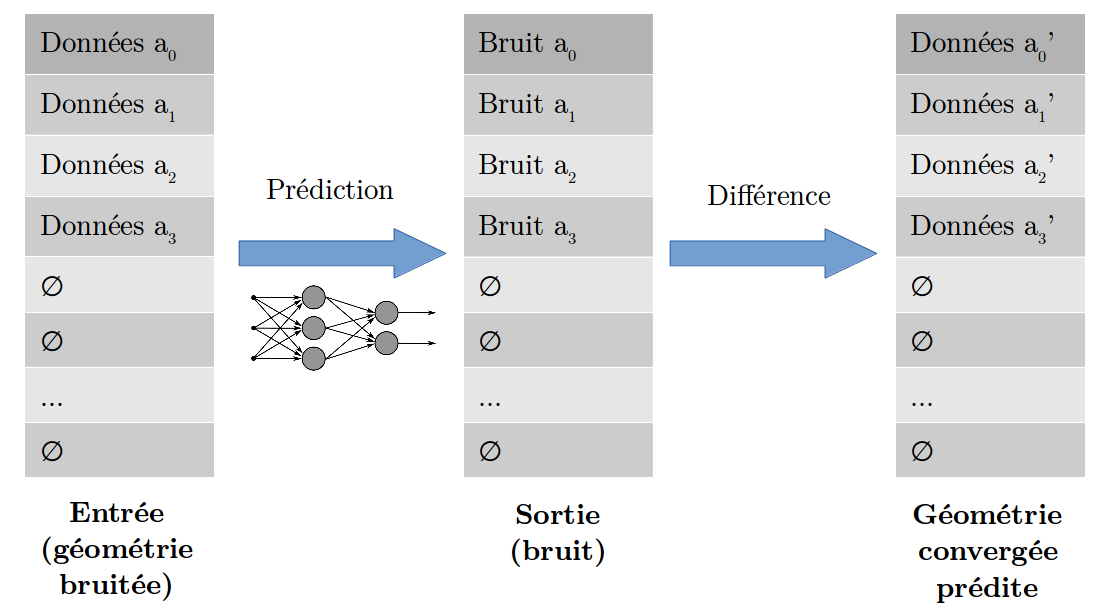
\includegraphics[scale=0.35]{images/flux_donnees.png}
	
	\caption{Flux de données des modèles \emph{DELTA\_DIST+H} pour une molécule de taille 4}
	\label{fig_flux}
\end{figure}
